\documentclass{article}
\usepackage{tabularx}
\usepackage{amsmath}
\usepackage{graphicx}
\usepackage[margin=2cm]{geometry}
\usepackage{cite}
\usepackage[final]{hyperref}
\usepackage{listings}
\usepackage{here}
\hypersetup{
	colorlinks=true,
	linkcolor=blue,
	citecolor=blue,
	filecolor=magenta,
	urlcolor=blue         
}

\begin{document}

\title{TP08\\Vulkan synchronisation}
\author{Robin Faury}
\date{02/19/20}
\maketitle

\begin{abstract}
	In this practical work, we will see how to run two compute shader with a write/read safe. There is two kind of synchronisation. The memory and the thread synchronisation. For the first one we will wait the end of the first compute shader before reading the buffer filled. For the other one we will duplicate the buffer to avoid write/read when we will want to read neighborhood.
\end{abstract}

\section{Post effect - Linear blur}
We want for some reason blur our outputed image. Modify your shader to apply this kernel at the end of the fractal generation. Out of image border will be ignored.

\begin{figure}[H]
	\centering
	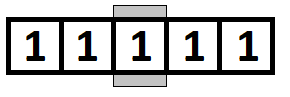
\includegraphics[scale=0.9]{figures/kernel_blur.png}
	\caption{Kernel for linear blur}
\end{figure}

The output may be good but you can see artefacts like those:

\begin{figure}[H]
	\centering
	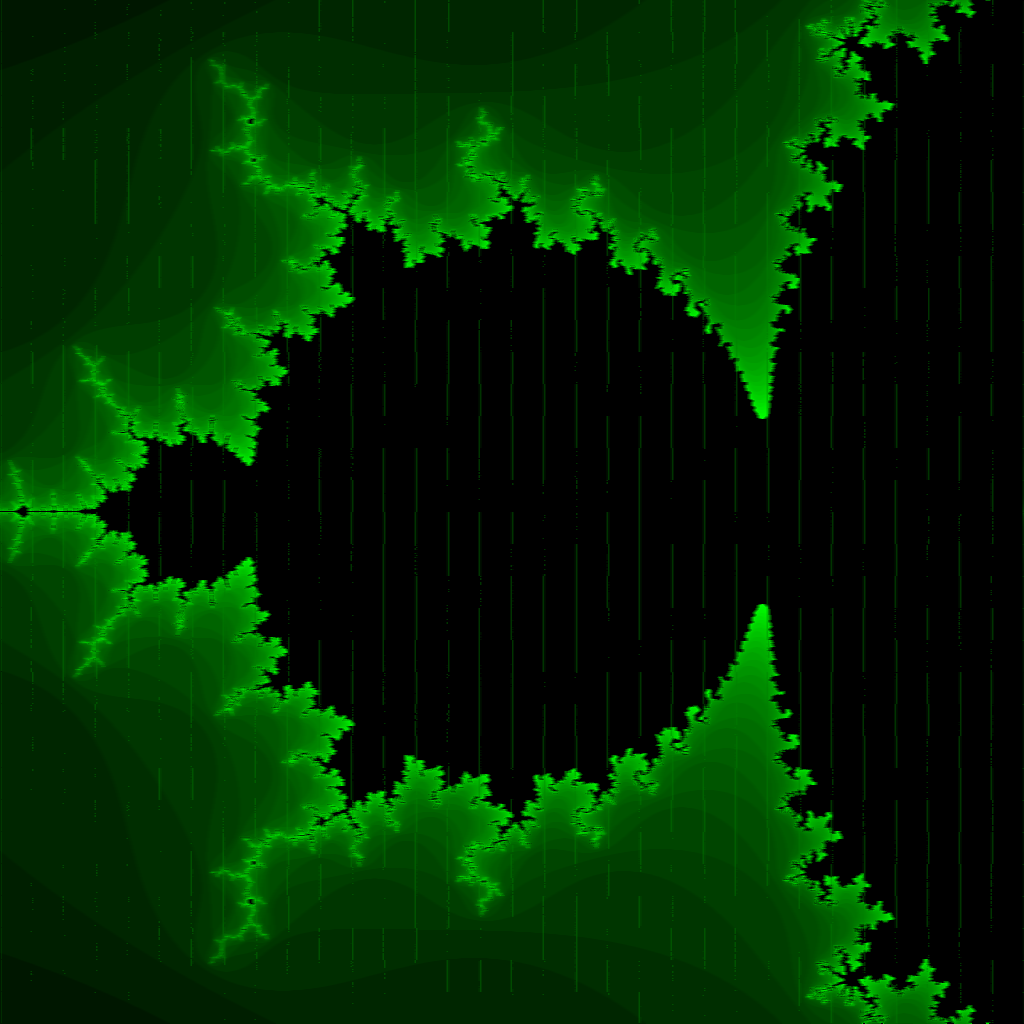
\includegraphics[scale=0.24]{figures/Mandelbrot_issues.png}
	\caption{Mandelbrot set computed on GPU}
\end{figure}

This happen because we read some date while there are computed. We need to wait each shader invocations before reading the neighborhood.

\section{synchronisation}
We saw having one shader with a write and read behaviours cause artefact. So we need two compute shaders:

\begin{itemize}
	\item The fractal generation
	\item The post effect
\end{itemize}

Create another compute shader to apply the post effect, its VkShaderModule and its VkPipeline. Fortunately, we can reuse all other object needed for the creation of the shader module and the pipeline because any layout has been changed. During the recording of command, simply bind the new pipeline, its descriptor set, its push constants and call its dispatch in the same way that the previous one. On the Vulkan specification, it's said that commands is executed in order, but they might finish out of order. That mean if your first shader is slow you may still having artefact.

\subsection{Memory Barrier}
In this section we will see how to use memory synchronisation. Barrier is the Vulkan system used for synchronisation. Right after the first dispatch we will create a memory barrier and we will add it to the command buffer:

\begin{lstlisting}
	VkMemoryBarrier memoryBarrier = {};
	memoryBarrier.sType = VK_STRUCTURE_TYPE_MEMORY_BARRIER;
	memoryBarrier.srcAccessMask = VK_ACCESS_SHADER_WRITE_BIT;
	memoryBarrier.dstAccessMask = VK_ACCESS_SHADER_READ_BIT;

	vkCmdPipelineBarrier(
		commandBuffer,
		VK_PIPELINE_STAGE_COMPUTE_SHADER_BIT,
		VK_PIPELINE_STAGE_COMPUTE_SHADER_BIT,
		0,
		1,
		&memoryBarrier,
		0, nullptr, 0, nullptr);
\end{lstlisting}

This barrier force a synchronisation between the two compute shaders. For your information, inside a big pipeline a lot of optimisation can be done with barrier.\\
To test this barrier use a very simple post effect like invert the red and the green. Without the barrier you may try to apply a post effect on a pixel not computed yet.

\subsection{In Out Buffer}
For the linear blur we need to read neighborhood pixel. We saw how to write and read on the same buffer using two shader, but here we should read and write on the same shader. We need a thread synchronisation.

\begin{enumerate}
	\item read neighborhood for each shader invocation
	\item wait each shader invocation finnished
	\item write the current pixel
\end{enumerate}

\begin{figure}[H]
	\centering
	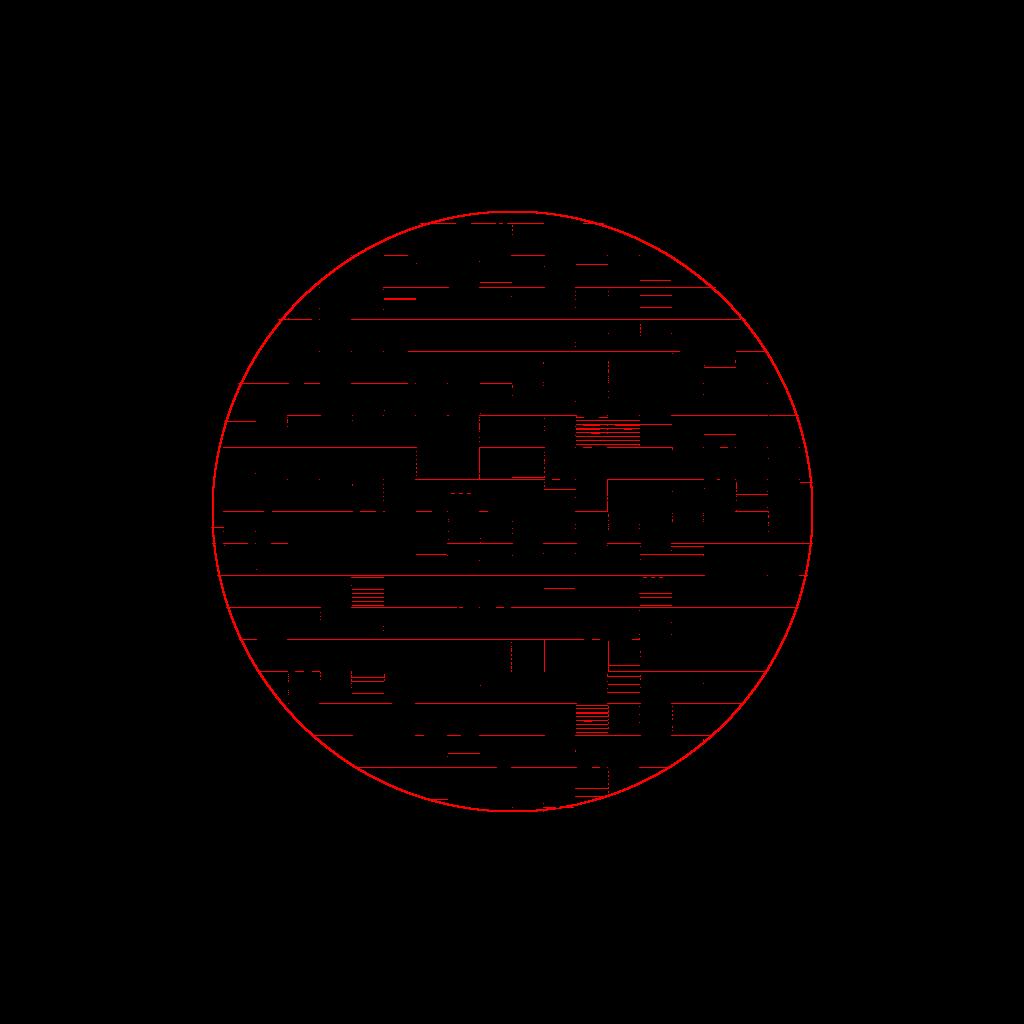
\includegraphics[scale=0.3]{figures/sobel.png}
	\caption{Sobel image processing without thread synchronisation}
\end{figure}

Unfortunately, Vulkan don't allow us to do that. The solution is to use two buffers. Create another GPUBuffer called GPUBufferOut with the same parameters as GPUBuffer. Modify the layout of your shader to bind two buffer on your compute shader. You can now read any pixel from the first buffer and populate the second.

\section{Image processing}
We can now create an image processing libriary. Create a shader to generate a circle and another one to apply the sobel filter.

\begin{figure}[H]
	\centering
	
\includegraphics[scale=1]{figures/sobel_kernel.png}
	\caption{Sobel kernel}
\end{figure}

For each pixel apply this formula to get edge detection: $G = abs(G_x) + abs(G_y)$

\end{document}